\section{Approach Overview}
\label{overview:sec}

\begin{figure}[t]
	\centering
	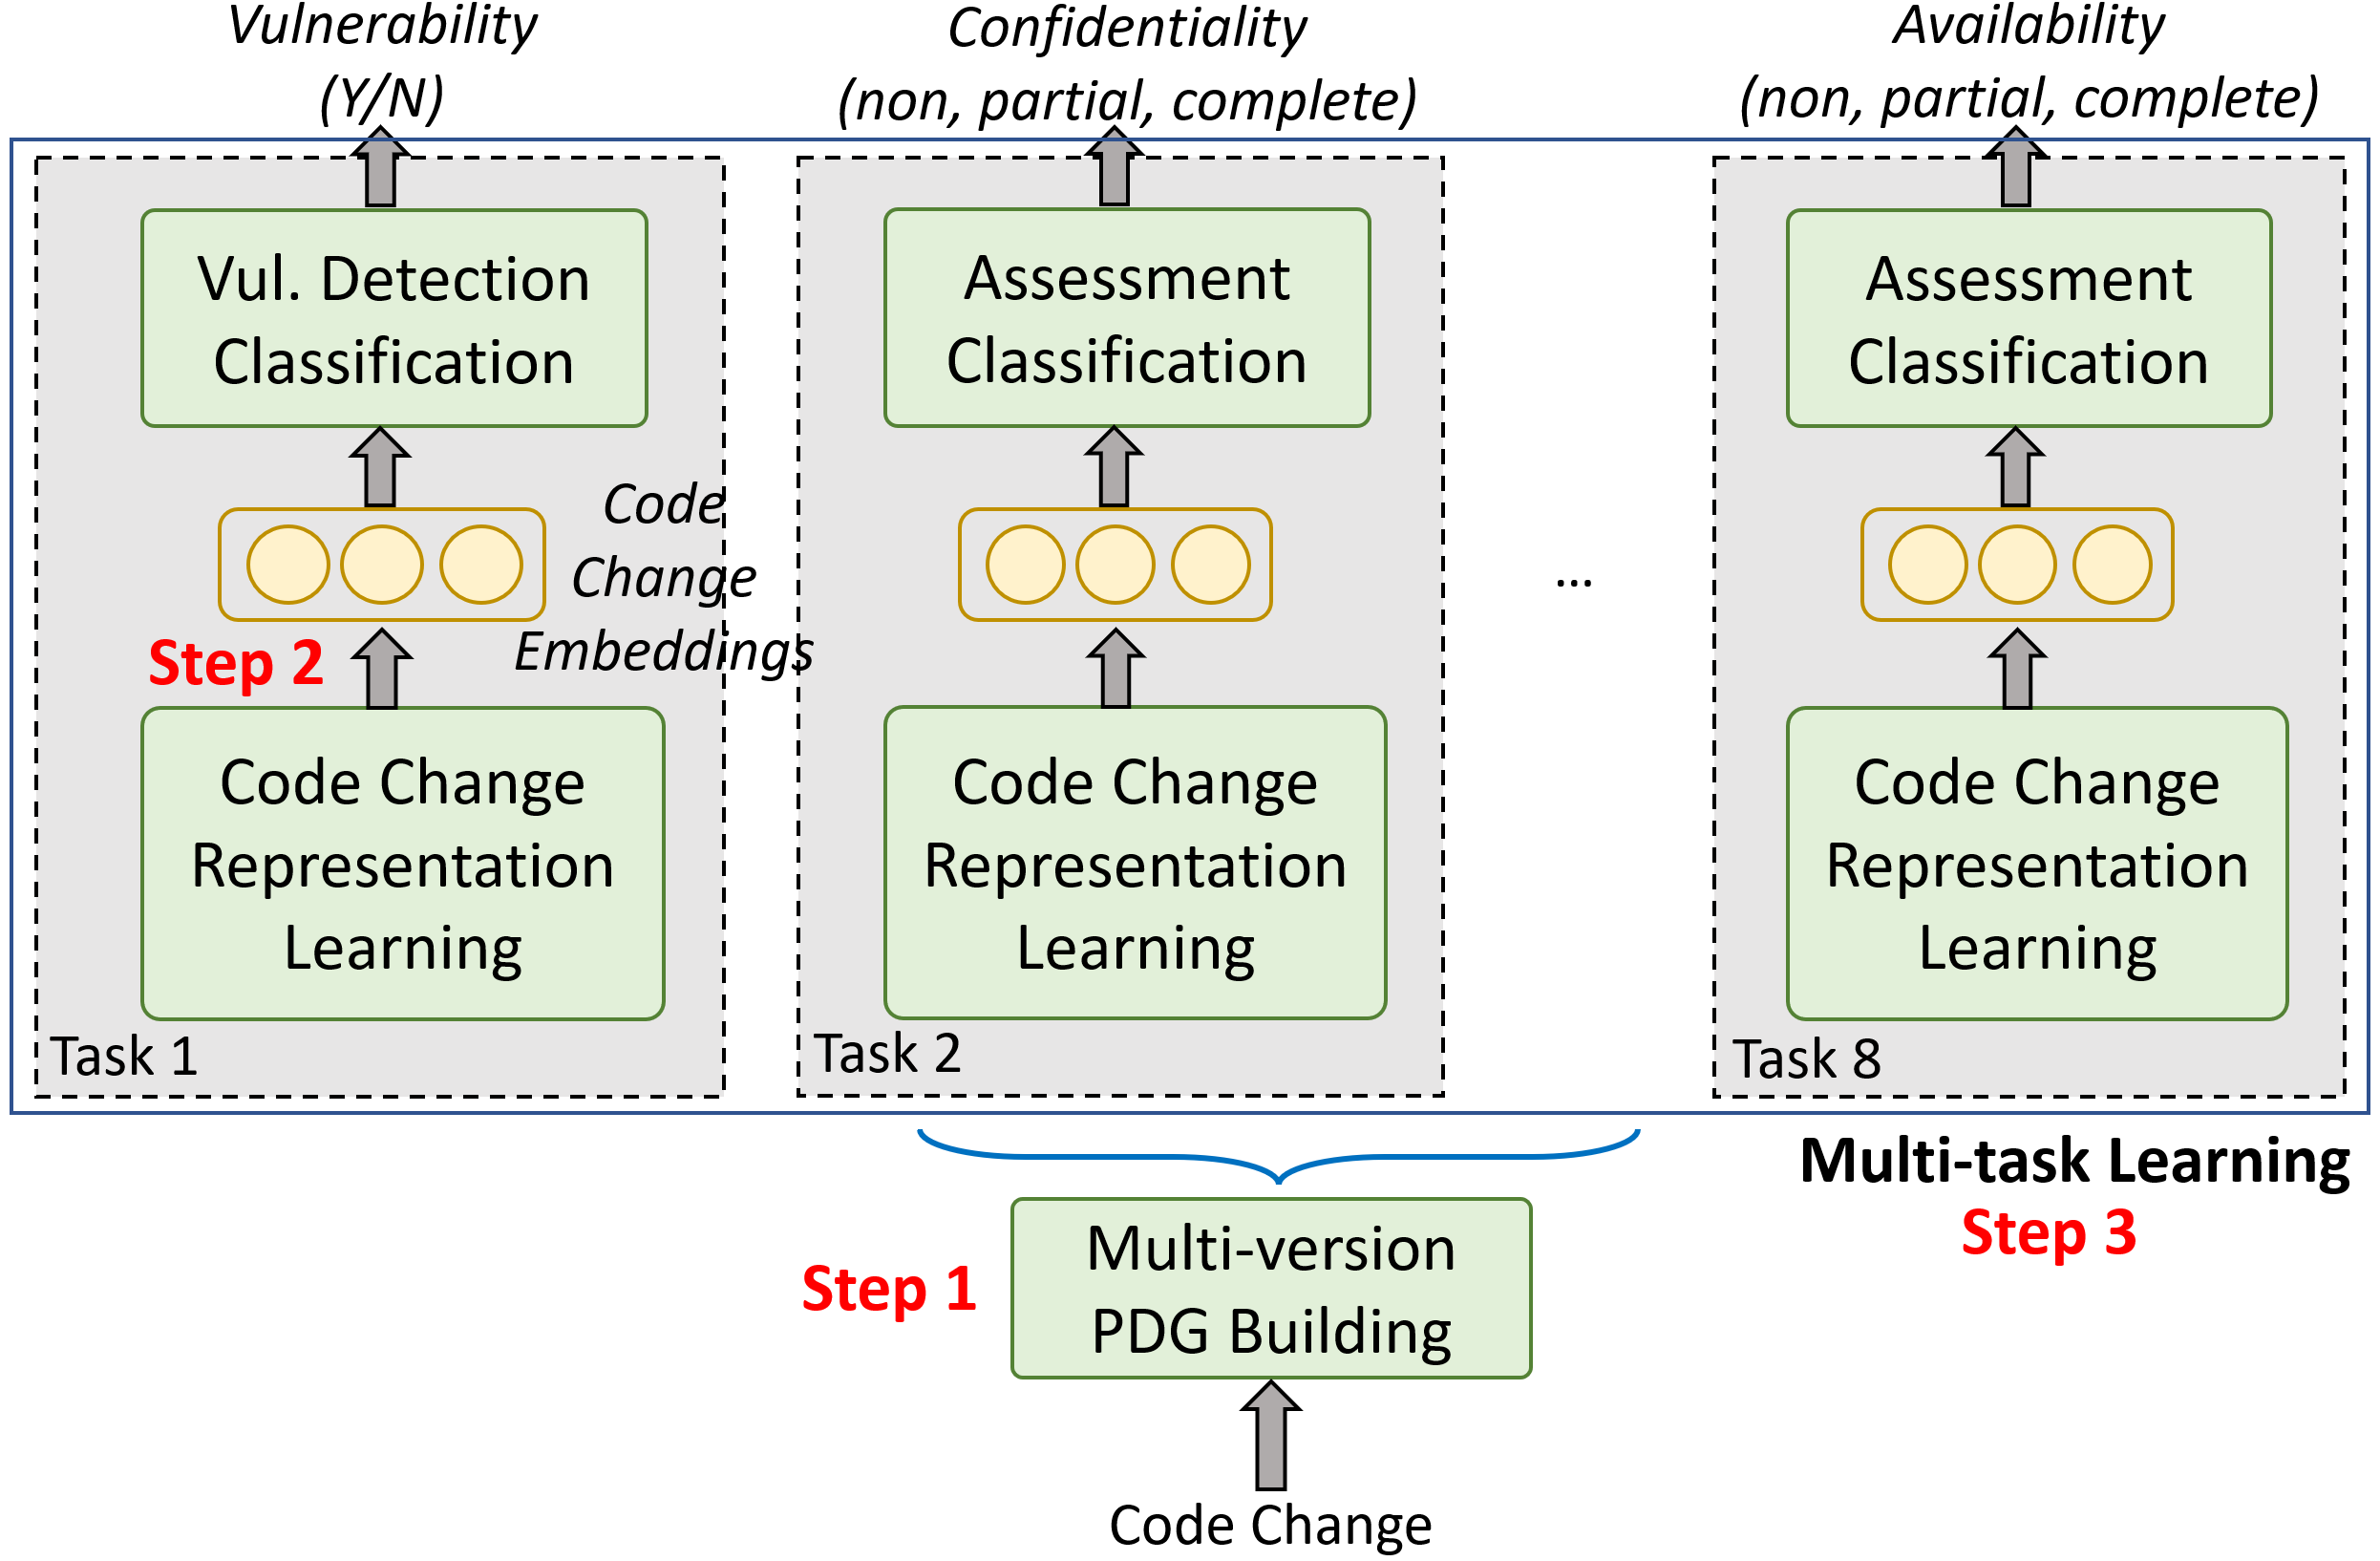
\includegraphics[width=3.4in]{graphs/overview-4.png}
	\vspace{-16pt}
	\caption{{\tool}: Context-aware, Graph-based, Commit-level
Vulnerability Detection and Assessment}
	\label{fig:overview}
\end{figure}

%Figure~\ref{fig:overview} illustrates the overall architecture of
%{\tool}.

\noindent {\tool} has three key components working in three~steps
(Figure~\ref{fig:overview}).

%\subsubsection*{{\bf Step 1. Multi-version PDG ({\mvpdgxy}) Generation}}

%\vspace{2pt}

\subsubsection*{{\bf Step 1. Representing Code Changes and Contexts with Multi-version PDG}}
Program Dependence Graph (PDG)~\cite{pdg} is a directed graph with a
set $N$ of nodes and a set $E$ of edges, in which a node $n \in N$
represents a program statement or a conditional expression; an edge $e
\in E$ represents the data or control flow among the statements.
%We adopt a graph representation, called
We adopt {\em the multi-version PDG ({\mvpdgxy})~\cite{flexeme-fse20} to
represent the changes between two versions $x$ and $y$, before and
after the commit}.  A multi-version PDG {\mvpdgxy}~\cite{flexeme-fse20}
is a directed graph generated from the disjoint union of all nodes and
edges in the PDGs at versions $x$ and~$y$. {\mvpdgxy}
(Figure~\ref{fig:multi-version-pdg}, Section~\ref{delta:sec}) allows
us to capture the program dependencies including data/control flows
that are crucial in vulnerability detection and assessment (Key
idea~2).

%\begin{Definition}[Multi-version Program Dependence Graph] ({\bf {\mvpdgxy}}).
%A {\mvpdgxy}~\cite{flexeme-fse20} is a directed graph generated from the
%disjoint union of all nodes and edges in the PDGs at versions $x$
%and~$y$.
%\end{Definition}

%{\mvpdgxy} is a directed graph generated from the disjoint union of
%all nodes and edges in both PDGs at the version $x$ and the version
%$y$ (Figure~\ref{fig:multi-version-pdg}).



%Contextualized Embeddings for Code Changes

%\vspace{2pt}

\subsubsection*{{\bf Step 2. Contextualized Embeddings for Code Changes with
    Graph-based Representation Learning}}
We develop our representation learning model to learn the
contextualized embeddings for the code changes in a commit that
integrate both program dependencies and the contexts. To build the
contextualized embeddings, we leverage the Label, Graph-based
Convolution Network~\cite{label-gcn} to learn the vector $v$ for each
node $n$ in the graph whose nodes can have labels. We use labels to
denote the nodes at either the versions $x$ (before changes) or $y$
(after changes), or at both versions.

For a changed node $n_c$, we collect all the un-changed nodes in the
context of $n_c$, which is defined as the set of all the un-changed
nodes that are $k$-hop neighbors of $n_c$. In
Figure~\ref{fig:multi-version-pdg}, for the changed statement at line
4, if $k=1$, the context of that change includes the statements at
lines 2, 5, and 7 (i.e., 1-hop neighbors from line 4).

From the context nodes, we compute the vector for the context for a
changed node $n_c$ and use it as a weight to represent the impact of
context to build the contextualized embedding for $n_c$.  From those
embeddings, we compute the vector for the entire commit and feed it to
a SoftMax layer acting as a classifier to perform vulnerability
classification or assessment classification for each assessment
type. The softmax function is often used as the last activation
function of a neural network to normalize the output of a network to a
probability distribution over the predicted output classes.

%Tien rewrote this para as above
%We collect the vectors of the context nodes into a matrix and use a
%fully connected layer to convert the matrix into a vector $v_{ctx}$ to
%encode the contextual information for the changed node $n_c$. The
%context vector $v_{ctx}$ is used as a weight to represent the impact
%of context on learning to build the contextualized embedding for the
%changed node $n_c$. We next concatenate all the vectors for the all
%the changed nodes $n_c$s into a matrix and use a fully connected layer
%to build the final vector $v^{com}$ for the entire commit. Finally, we
%feed the vector $v^{com}$ to a SoftMax layer acting as a classifier to
%perform assessment classification for each CVSS assessment type.


%\subsubsection{{\bf Step 2. Multi-task Learning-based Vulnerability Assessment Classification}}

%After having the {\mvpdgxy}, this step is mainly used to do the classification for seven different vulnerability assessment types. To achieve that, \tool setups seven separate but similar tasks on seven vulnerability assessment classification problems. Here, we pick one task to explain it in detail.

%The first step of the vulnerability assessment classification is to learn the summarized representation vector for the code changes in the vulnerability bring commit. In this step, \tool uses the Label-GCN \cite{} that can deal with the nodes with multiple labels (suitable for $x$, $y$, and $x,y$ labels in {\mvpdgxy})to learn the representation vector $v$ for each node $n$ in the graph. \tool then picks out all changed nodes in {\mvpdgxy} as a set. For each changed node $n^c$ in this set, \tool firstly collects the representation vector $v^{uc}$ for all unchanged nodes $n^{uc}$ within the $k$-hops in {\mvpdgxy} as the context of the changed node $n^c$. For example, in the {\mvpdgxy} in Figure \ref{fig:multi-version-pdg}, if we regard the statement in $line-4$ is the changed statement that we are focusing on. When $k=1$, the context of it includes the statements in $line-2$, $line-5$, and $line-7$. By concatenating $v^{uc}$ in a new dimension as a matrix, \tool uses a fully connected layer to summarize the matrix into one vector $v^{ctx}$ to represent the context information for the changed node $n^c$. Then, \tool uses the cross product to combine the node representation vector $v^c$ with the context representation vector $v^{ctx}$ to get the final representation vector $v'^c$ for the changed node $n^c$.


%Because the vulnerability assessment we want to get is for the whole vulnerability bring in commits, \tool concatenates $v'^c$ as a matrix and uses a fully connected layer to summarize the final code change representation vector $v^{commit}$. After having the final code change representation vector $v^{commit}$, \tool uses the SoftMax layer as a classifier to do the vulnerability assessment classification based on the $v^{commit}$.

%\vspace{2pt}
\subsubsection*{{\bf Step 3. Multi-Task Learning for Classification}}

For each assessment type, we~have a SoftMax layer working as an
assessment classification model on the embedding of the entire commit.
We also have another SoftMax layer as the classifier for
vulnerability detection.
%
%the SoftMax layer acts as the classifier, which takes
%the~contextualized embedding for the entire commit built on the
%{\mvpdgxy} and performs classifications.
%
To propagate the impact of the classification for one assessment type
on one another, we leverage multi-task learning among all the
classification models. We use the uncertainty weighted multi-task
loss~\cite{kendall2018multi} for each classification task as the final
multi-task learning loss function and use the maximum of the average
F-score from all the classification tasks as the training~target.

%After \tool has seven different classification tasks as we introduced above, \tool uses the weighted linear sum of the losses for each task as the final multi-task learning loss function and uses the maximum of the average F-1 score from all vulnerability assessment classification tasks as the training target to train the model.

%When making a prediction, based on the requirements, \tool can directly provide classification results for a single vulnerability assessment type or multiple vulnerability assessment types as needed.

%Training and Predicting process

\subsubsection*{{\bf Training and Predicting Processes}}
The training and predicting processes share the above steps, except
that in training, the classification labels for the vulnerable commit
and vulnerability assessment types (VATs) are known. For a benign
commit, the output labels are negative and non-impact.
%vulnerability-introducing commits w.r.t. a VAT are known.
When predicting, {\tool} takes a code change, predicts
vulnerability and provides the assessment classifications for seven
VATs. Next, we will explain {\tool} in details.

%directly provide classification results for a single vulnerability
%assessment type or multiple vulnerability assessment types as needed.


%fix the figure
